\documentclass{article}
\usepackage[pdfcreator={LaTeX}]{hyperref}
\usepackage{graphicx}
\usepackage[utf8]{inputenc} 
\usepackage[ngerman]{babel}


\usepackage{tikz}
\usetikzlibrary{arrows,shadows}
\usepackage{pgf-umlsd}


\begin{document}
\begin{titlepage}

\begin{center}
\textbf{\textsc{\LARGE Implementierungsbericht}}

{\large \today}

\vspace{2cm}
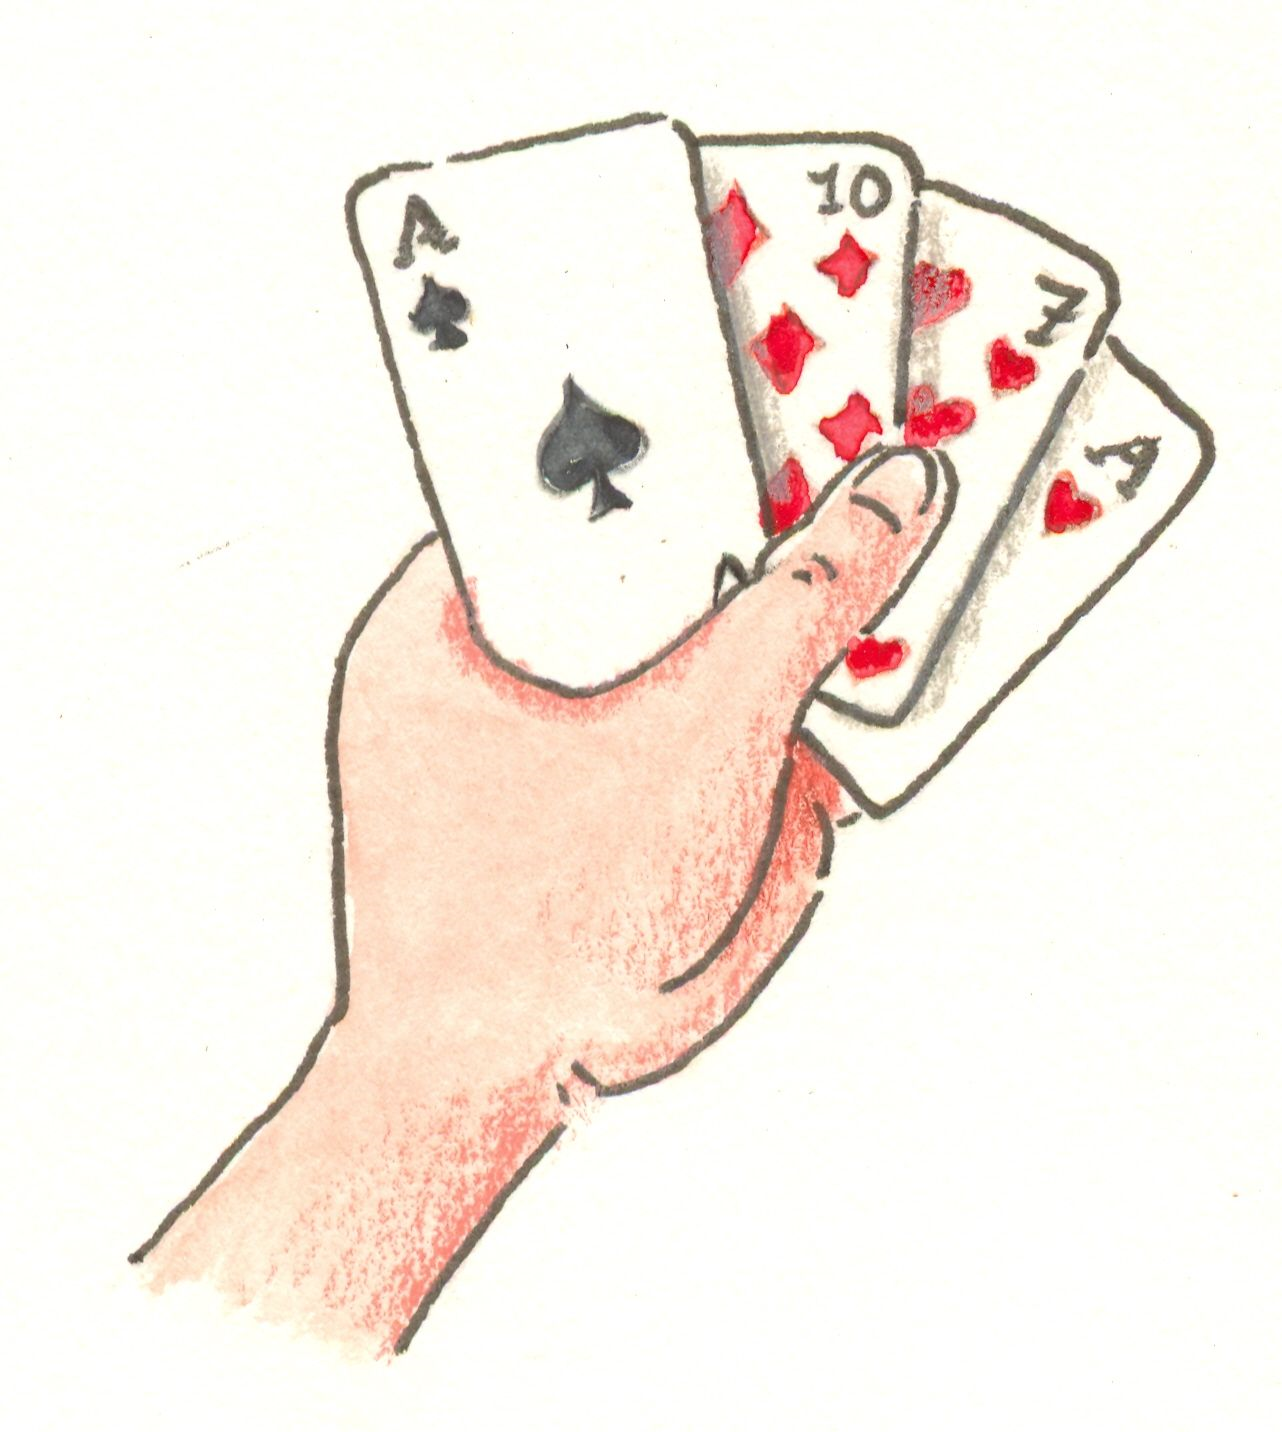
\includegraphics{kartenspiel}
\ \\
\ \\

\textbf{\textsc{\LARGE NET-WizHearts}}
\vspace{2cm}

\begin{tabular}{|c|c|c|}\hline
   Phase & Verantwortlicher & E-Mail \\ \hline\hline
   Pflichtenheft & Alina Meixl &  alina@meixl.de \\ \hline
   Entwurf & Viktoria Witka & witkaviktoria@freenet.de \\ \hline
   Spezifikation & Daniel Riedl & dariedl14@yahoo.de \\ \hline
   Implementation & Andreas Altenbuchner& a.andi007@gmail.com\\ \hline
   Verifikation & Patrick Kubin & kubin@fim.uni-passau.de\\ \hline
   Präsentation & w& w\\ \hline
 \end{tabular}

\end{center}

\end{titlepage}

\tableofcontents
\newpage

\section{Einleitung}
Hier kommt die Implementierung

\newpage

\section{Änderungen gegenüber der Spezifikation}

\subsection{Client}

\begin{itemize}
\item  \textbf{LanguageInterpreter:}  \textit{Neu hinzugefügte Klasse}: Wird verwendet, um Fehlermeldungen, die vom Server gesendet werden zu interpretieren und in der korrekten Sprache auszugeben.
\end{itemize}

\subsection{View}

\begin{itemize}
\item \textbf{Login:} \textit{hinzugefügt}: getUsername(), getServerAdress()
\item \textbf{Lobby:} \textit{hinzugefügt}: getChosenGameName(), getChatMessage(), hasPWChosenGame()
\item \textbf{CreateWindow:} \textit{entfernt}: addLeaveButtonListener(), addRulesetSelectionListener(); \textit{hizugefügt}: setRulesetTypes(), getGameName(), hasPassword(), getPassword(), getSelectedRulesetType()
\item \textbf{GameLobby:} \textit{hinzugefügt}: getChatMessage(), getSelectedPlayer()
\end{itemize}

\subsection{Ruleset}

\begin{itemize}
\item \textit{hinzugefügt} \textbf{DiscardedCard:} ;

\item \textit{hinzugefügt} \textbf{EmptyCard:};

\item \textbf{WizardCard:} \textit{hinzugefügt}: changeSorcererColour ();

\item \textbf{GameState:} \textit{hinzugefügt}: madeTrick(), restartDeck (), newRound(); \textit{gelöscht}:getNumberOfPlayedCards(), getCardsLeftInDeck()

\item \textbf{ServerWizard:} \textit{hinzugefügt}: updatePlayers (), getPlayedCards (),
startRound(); 

\item \textbf{ServerHearts:} \textit{hinzugefügt}: swapLeft(),swapRight(),swapAcross(), swap
\textit{geändert}: getWinners(),  ;
\end{itemize}

\subsection{Server}

\begin{itemize}
\item  \textbf{LoginServer:}  \textit{Neu hinzugefügte Klasse, erbt von Server}: Sie ist für das Zustabdekommen von Clientverbindungen zuständig. \textit{Attribute}:  Thread clientListenerThread,  LobbyServer lobby; \textit{Methoden}: receiveMessage(Player player, ComLoginRequest login), disconnectPlayer()
\item  \textbf{GameServer:} \textit{hinzugefügt}: quitGame(), getGameMasterName(), getPassword(), sendRulesetMessage(String player, RulesetMessage message), broadcastRulesetMessage(RulesetMessage message), sendWarning(String player, WarningMsg warning), broadcastWarning(WarningMsg warning)
\item  \textbf{GameServerRepresentation:} \textit{implementiert jetzt Serializable}
\item  \textbf{LobbyServer:} \textit{entfernt}: innere Klasse ClientListenerThread, Set<Player> noNames, ServerSocket socket, receiveMessage(Player player, ComClientQuit quit ), receiveMessage(Player player, ComLoginRequest login); \textit{hinzugefügt}: addPlayerToGame(Player player, GameServer game), getNames()
\item  \textbf{ClientListenerThread:} erbt jetzt von Thread  \textit{hinzugefügt}: boolean waiting, ServerScocket socket, LoginServer server
\item  \textbf{Player:}  erbt jetzt von Thread  \textit{hinzugefügt}: Socket connection, boolean run, closeConnection(); \textit{geändert}: getName() heißt getPlayerName(), setName() heißt setPlayerName()
\item  \textbf{Server:} \textit{hinzugefügt}: eine receiveMessage Methode für jedes ComObject, das vom Server empfangen werden soll; \textit{geändert}: handleIOException heißt jetzt disconnectPlayer()
\item  \textbf{ServerMain:} \textit{hinzugefügt}: Attribut LoginServer loginServer
\end{itemize}

\subsection{ComObjects}

\begin{itemize}
\item 
\end{itemize}

\newpage

\section{Vergleich: Implementierungsplan und Realität}

\subsection{Änderungen am Plan}
\begin{itemize}
\item Zuständigkeit von Arbeitspaket Client(Lobby) wurde von Patrick an Andi gegeben, um die Arbeitszeiten anzugleichen
\item Zuständigkeit von Arbeitspaket Ruleset(Wizard-Client) wurde von Patrick/Andi and Daniel gegeben, um die Arbeitszzeiten anzugleichen
\end{itemize}

\subsection{Milestone 1}

\begin{itemize}
\item \textbf{View(Login+Lobby):} ang. Dauer: 8 Stunden, tats. Dauer: 4 Stunden \\
Begründung: Es waren noch Code-Teile aus der Pflichtenheft-Phase vorhanden. \\
\item \textbf{View(Create+Join):} ang. Dauer: 8 Stunden, tats. Dauer: 4 Stunden \\
\item \textbf{View(GameLobby):} ang. Dauer: 8 Stunden, tats. Dauer: bisher 3 Stunden \\
\item \textbf{Model(Login):} ang. Dauer: 8 Stunden, tats. Dauer: bisher 8.5 Stunden \\
Begründung: Login mehrmals umgebaut um die Tests aus dem Pflichtenheft zu erfüllen. \\
\item \textbf{Model(Lobby):} ang. Dauer: 8 Stunden, tats. Dauer: bisher 6.5 Stunden \\
\item \textbf{Model(Create+Join):} ang. Dauer: 8 Stunden, tats. Dauer: bisher 6 Stunden \\
\item \textbf{Server(Login):} ang. Dauer: 16 Stunden, tats. Dauer: 6 Stunden \\
Begründung: Viele der ComObjects waren bereits fertig.
\item \textbf{Server(Lobby):} ang. Dauer: 8 Stunden, tats. Dauer: 3 Stunden 
\item \textbf{Server(Create+Join):} ang. Dauer: 12 Stunden, tats. Dauer: 6 Stunden 
\item \textbf{Ruleset(Daten):} ang. Dauer: 20 Stunden, tats. Dauer: 5 Stunden
Begründung: Wurde hauptsächlich schon in Spezifikationsphase implementiert

\item \textbf{Ruleset(ServerWizard):} ang. Dauer: 30 Stunden, tats. Dauer: 20 Stunden

\item \textbf{Ruleset(ServerHearts):} ang. Dauer: 30 Stunden, tats. Dauer: bisher 6 Stunden
\item \textbf{Ruleset(ClientWizard):} ang. Dauer:6 Stunden, tats. 
Dauer: bisher 3 Stunden
\end{itemize}

\subsection{Milestone 2}
\item \textbf{Server(GameLobby):} ang. Dauer: 10 Stunden, tats. Dauer: 5 Stunden 

\subsection{Milestone 3}
\item \textbf{Server(Game):} ang. Dauer: 4 Stunden, tats. Dauer: 2 Stunden 30 Minuten
 
\subsection{Finale Phase}




\end{document}
